\subsubsection{The ``Stokes' law'' benchmark}
\label{sec:benchmark-stokes_law}

\textit{This section was contributed by Juliane Dannberg.}

Stokes' law was derived by George Gabriel Stokes in 1851 and describes the frictional force
a sphere with a density different than the surrounding fluid experiences in a
laminar flowing viscous medium.
A setup for testing this law is a sphere with the radius $r$ falling in a highly
viscous fluid with lower density. Due to its higher density the sphere is
accelerated by the gravitational force. While
the frictional force increases with the velocity of the falling particle,
the buoyancy force remains constant. Thus, after some time the forces will
be balanced and the settling velocity of the sphere $v_s$ will remain constant:

\begin{align}
  \label{eq:stokes-law}
  \underbrace{6 \pi \, \eta \, r \, v_s}_{\text{frictional force}} =
  \underbrace{4/3 \pi \, r^3 \, \Delta\rho \, g,}_{\text{buoyancy force}}
\end{align}
where $\eta$ is the dynamic viscosity of the fluid, $\Delta\rho$ is the
density difference between sphere and fluid and $g$ the gravitational
acceleration. The resulting settling velocity is then given by
\begin{align}
  \label{eq:stokes-velo}
  v_s = \frac{2}{9} \frac{\Delta\rho \, r^2 \, g}{\eta}.
\end{align}
Because we do not take into account inertia in our numerical computation,
the falling particle will reach the constant settling velocity right after
the first timestep.

For the setup of this benchmark, we chose the following parameters:
\begin{align*}
  \label{eq:stokes-parameters}
  r &= 200 \, \si{km}\\
  \Delta\rho &= 100 \, \si{kg}/\si{m}^3\\
  \eta &= 10^{22} \, \si{Pa.s}\\
  g &= 9.81 \, \si{m}/\si{s}^2.
\end{align*}
With these values, the exact value of sinking velocity is $v_s =
\num{8.72e-10} \, \si{m}/\si{s}$.

To run this benchmark, we need to set up an input file that describes the
situation. In principle, what we need to do is to describe a spherical object
with a density that is larger than the surrounding material. There are multiple
ways of doing this. For example, we could simply set the initial temperature of
the material in the sphere to a lower value, yielding a higher density with any
of the common material models. Or, we could use \aspect{}'s facilities to advect
along what are called ``compositional fields'' and make the density dependent on
these fields.

We will go with the second approach and tell \aspect{} to advect a single
compositional field. The initial conditions for this field will be zero outside
the sphere and one inside. We then need to also tell the material model to
increase the density by $\Delta\rho=100 kg\, m^{-3}$ times the concentration of
the compositional field. This can be done, like everything else, from the input
file.

All of this setup is then described by the following input file.
(You can find the input file to run this cookbook example in
\url{cookbooks/stokes/stokes.prm}. For your first runs you will probably want to
reduce the number of mesh refinement steps to make things run more quickly.)

\lstinputlisting[language=prmfile]{cookbooks/benchmarks/stokes/doc/stokeslaw.prm.out}

Using this input file, let us try to evaluate the results of the current
computations for the settling velocity of the sphere. You can visualize the output in different
ways, one of it being ParaView and shown in
Fig.~\ref{fig:stokes-falling-sphere-2d} (an alternative is to use Visit as
described in Section~\ref{sec:viz}; 3d images of this simulation using Visit
are shown in Fig.~\ref{fig:stokes-falling-sphere-3d}).
Here, ParaView has the advantage that you can calculate the average velocity
of the sphere using the following filters:
\begin{enumerate}
 \item Threshold (Scalars: C\_1, Lower Threshold 0.5, Upper Threshold 1),
 \item Integrate Variables,
 \item Cell Data to Point Data,
 \item Calculator (use the formula sqrt(velocity\_x\textasciicircum2+
       velocity\_y\textasciicircum2+velocity\_z\textasciicircum2)/Volume).
\end{enumerate}
If you then look at
the Calculator object in the Spreadsheet View, you can see the average sinking
velocity of the sphere in the column ``Result'' and compare it to the theoretical
value $v_s = \num{8.72e-10} \, \si{m}/\si{s}$.
In this case, the numerical result is $\num{8.865e-10} \,
\si{m}/\si{s}$ when you add a few more refinement steps to actually resolve
the 3d flow field adequately. The ``velocity statistics'' postprocessor we have
selected above also provides us with a maximal velocity that is on the same
order of magnitude. The difference between the analytical and the numerical
values can be explained by different at least the following three points:
(i) In our case the sphere is viscous and not rigid as assumed in Stokes' initial model, leading to
a velocity field that varies inside the sphere rather than being constant.
(ii) Stokes' law is derived using an infinite domain but we have a finite box
instead. (iii) The mesh may not yet fine enough to provide a fully converges
solution. Nevertheless, the fact that we get a result that is accurate to less
than 2\% is a good indication that \aspect{} implements the equations correctly.

\begin{figure}
  \begin{center}
    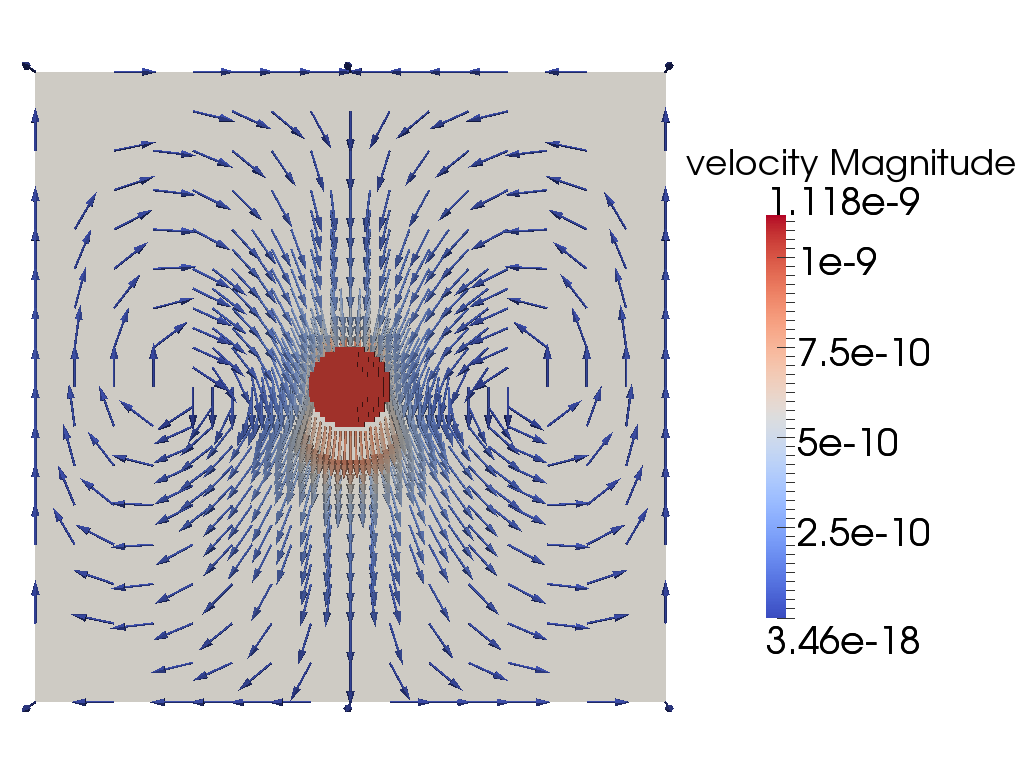
\includegraphics[width=0.55\textwidth]{cookbooks/benchmarks/stokes/doc/stokes-velocity.png}
    \hfill
    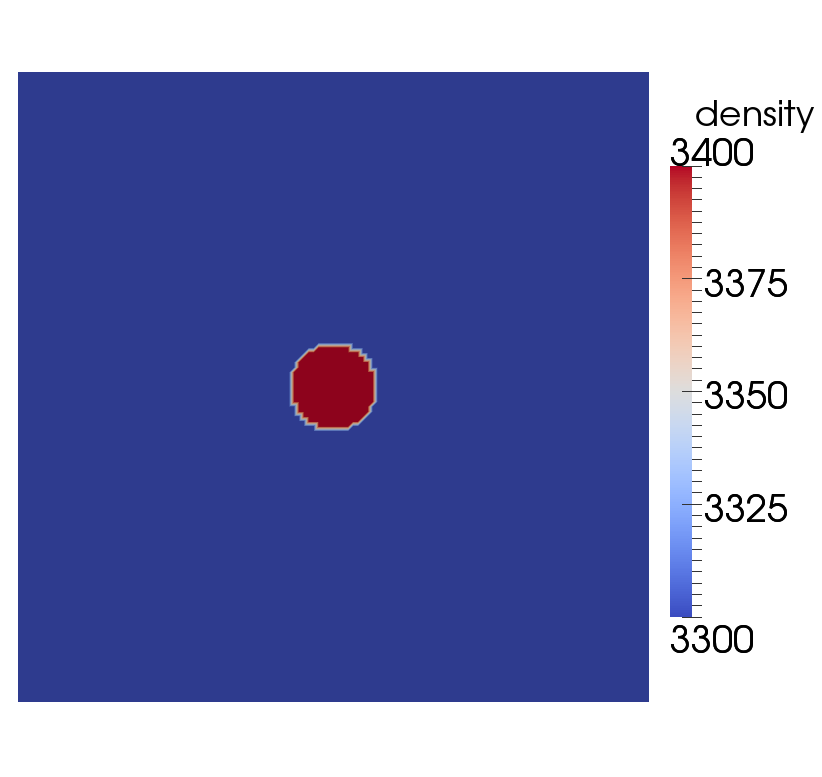
\includegraphics[width=0.44\textwidth]{cookbooks/benchmarks/stokes/doc/stokes-density.png}
  \end{center}
  \caption{\it Stokes benchmark. Both figures show only a 2D slice of the
      three-dimensional model.
      Left: The compositional field and overlaid to it some velocity vectors.
      The composition is 1 inside a sphere with the radius of 200 km and 0
      outside of this sphere. As the velocity vectors show, the sphere sinks
      in the viscous medium.
      Right: The density distribution of the model. The compositional density
      contrast of 100 kg$/\si{m}^3$ leads to a higher density inside of the
      sphere.}
  \label{fig:stokes-falling-sphere-2d}
\end{figure}

\begin{figure}
  \begin{center}
    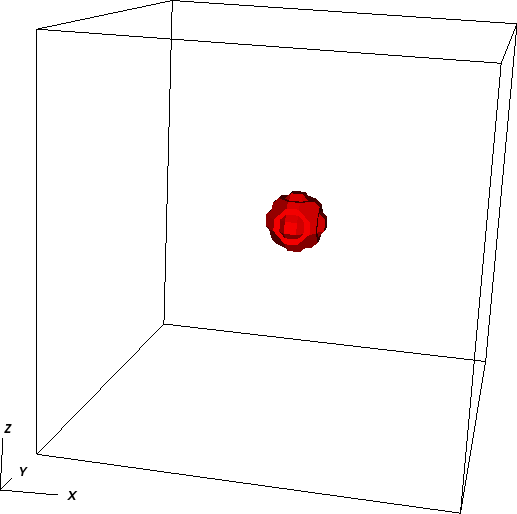
\includegraphics[width=0.3\textwidth]{cookbooks/benchmarks/stokes/doc/composition.png}
    \hfill
    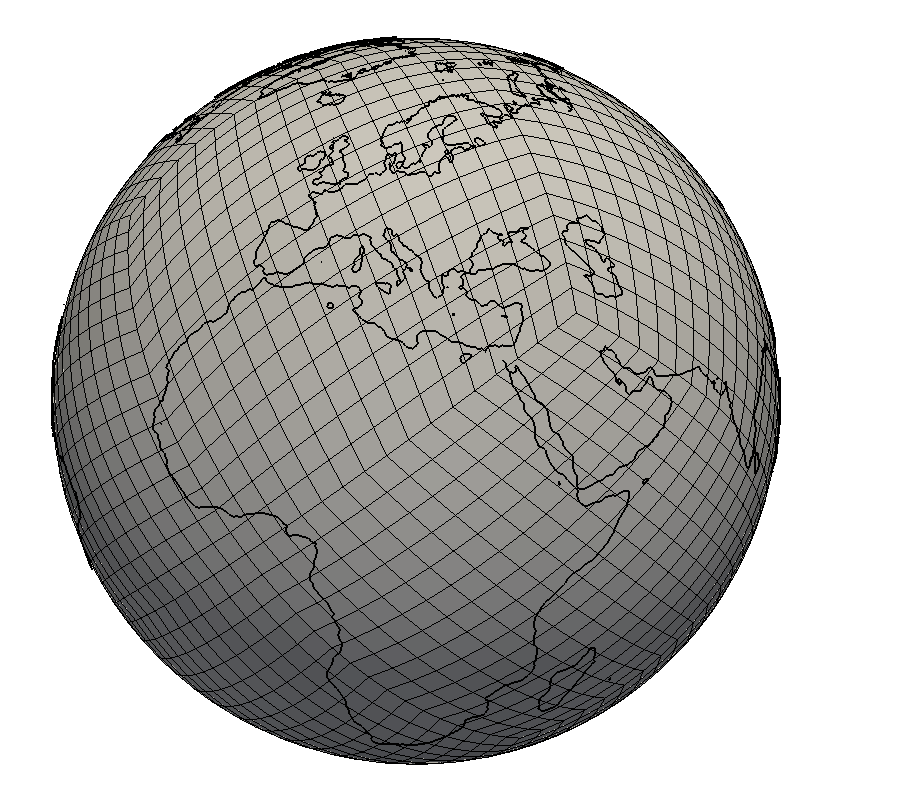
\includegraphics[width=0.3\textwidth]{cookbooks/benchmarks/stokes/doc/mesh.png}
    \hfill
    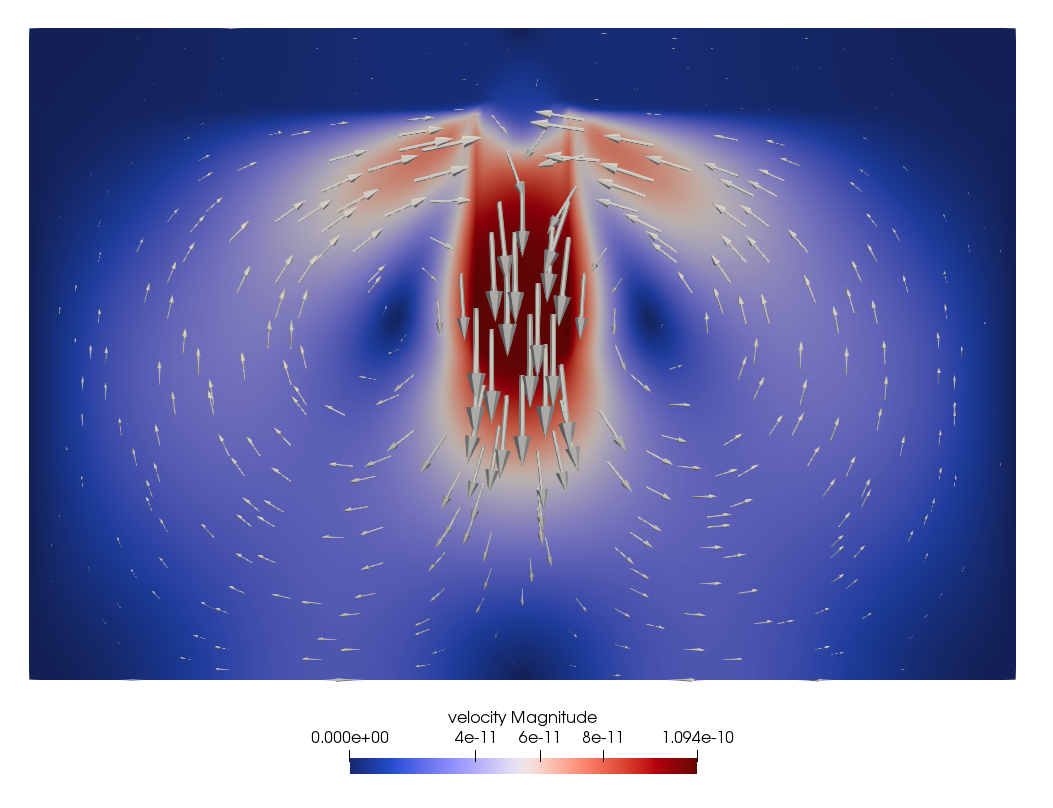
\includegraphics[width=0.3\textwidth]{cookbooks/benchmarks/stokes/doc/velocity.png}
  \end{center}
  \caption{\it Stokes benchmark. Three-dimensional views of the compositional
  field (left), the adaptively refined mesh (center) and the resulting velocity field
  (right).}
  \label{fig:stokes-falling-sphere-3d}
\end{figure}
